% =============================================================================
%  SICSS-BRAZIL 2026 — FGV/RIO DE JANEIRO
%  WORKSHOP DE ANÁLISE AUTOMATIZADA DE TEXTO (AUTOMATED TEXT ANALYSIS)
%  AULA 1 (MANHÃ) — ESTADO DA ARTE: EPISTEMOLOGIA, DESENHO E PRIMEIROS CÓDIGOS
%  Data: quarta-feira, 29 de julho de 2026 — 10h15 às 12h00 (105 minutos)
%  Facilitador: Anderson Henrique (CEM/USP · INCT QualiGov · IPEA)
%  Compilação: pdflatex (2 passes para resolver o TOC)
%  Figuras: pasta ./figuras (saídas ilustrativas)
%  Repositório: github.com/andersonheri/sicss-brazil-2026-text
% =============================================================================

\documentclass[11pt,aspectratio=169]{beamer}

% --- Codificação e idioma -----------------------------------------------------
\usepackage[utf8]{inputenc}
\usepackage[T1]{fontenc}
\usepackage[brazilian]{babel}
\usepackage{lmodern}

% --- Tema visual --------------------------------------------------------------
\usetheme{Madrid}
\usecolortheme{default}
\useinnertheme{rectangles}
\useoutertheme{miniframes}

\definecolor{azulUNI}{RGB}{31,78,121}
\definecolor{azulUNIclaro}{RGB}{68,114,150}
\definecolor{laranjaDestaque}{RGB}{200,90,30}
\definecolor{verdeCodigo}{RGB}{0,110,80}
\definecolor{cinzaCodigo}{RGB}{245,245,245}
\definecolor{cinzaSaida}{RGB}{237,240,243}

\setbeamercolor{structure}{fg=azulUNI}
\setbeamercolor{frametitle}{bg=azulUNI,fg=white}
\setbeamercolor{title}{bg=azulUNI,fg=white}
\setbeamercolor{section in head/foot}{bg=azulUNIclaro,fg=white}
\setbeamercolor{subsection in head/foot}{bg=azulUNI,fg=white}
\setbeamercolor{author in head/foot}{bg=azulUNI,fg=white}
\setbeamercolor{title in head/foot}{bg=azulUNIclaro,fg=white}
\setbeamercolor{date in head/foot}{bg=azulUNI,fg=white}

% Margens um pouco menores, para acomodar tabelas e diagramas
\setbeamersize{text margin left=0.55cm, text margin right=0.55cm}

% --- Pacotes auxiliares -------------------------------------------------------
\usepackage{tikz}
\usetikzlibrary{shapes.geometric,arrows.meta,positioning,calc,fit,backgrounds}
\usepackage{booktabs}
\usepackage{array}
\usepackage{amsmath,amssymb}
\usepackage{xcolor}
\usepackage{graphicx}
\usepackage{hyperref}
\usepackage{listings}

% --- Estilo para código R -----------------------------------------------------
\lstdefinestyle{Restilo}{
  language=R,
  basicstyle=\ttfamily\scriptsize,
  keywordstyle=\color{azulUNI}\bfseries,
  commentstyle=\color{verdeCodigo}\itshape,
  stringstyle=\color{laranjaDestaque},
  backgroundcolor=\color{cinzaCodigo},
  frame=single,
  rulecolor=\color{azulUNIclaro},
  breaklines=true,
  showstringspaces=false,
  numbers=none,
  columns=fullflexible,
  keepspaces=true,
  aboveskip=2pt, belowskip=2pt,
  literate={á}{{\'a}}1 {ã}{{\~a}}1 {â}{{\^a}}1 {é}{{\'e}}1 {ê}{{\^e}}1
           {í}{{\'i}}1 {ó}{{\'o}}1 {ô}{{\^o}}1 {õ}{{\~o}}1 {ú}{{\'u}}1
           {ç}{{\c c}}1 {Á}{{\'A}}1 {É}{{\'E}}1 {Í}{{\'I}}1 {Ó}{{\'O}}1
           {Ú}{{\'U}}1 {Ç}{{\c C}}1 {ü}{{\"u}}1
}
% --- Estilo para saída do console ---------------------------------------------
\lstdefinestyle{Rsaida}{
  basicstyle=\ttfamily\tiny\color{black!80},
  backgroundcolor=\color{cinzaSaida},
  frame=single,
  rulecolor=\color{black!25},
  breaklines=true,
  showstringspaces=false,
  numbers=none,
  columns=fullflexible,
  keepspaces=true,
  aboveskip=2pt, belowskip=2pt,
  literate={á}{{\'a}}1 {ã}{{\~a}}1 {é}{{\'e}}1 {í}{{\'i}}1 {ó}{{\'o}}1
           {õ}{{\~o}}1 {ú}{{\'u}}1 {ç}{{\c c}}1
}
\lstset{style=Restilo}

% --- Definições TikZ reutilizáveis -------------------------------------------
\tikzset{
  bloco/.style={rectangle, draw=azulUNI, thick, fill=azulUNI!10,
                rounded corners, minimum width=2.4cm, minimum height=0.85cm,
                align=center, font=\scriptsize},
  destaque/.style={rectangle, draw=azulUNI, very thick, fill=azulUNI!25,
                   rounded corners, minimum width=2.4cm, minimum height=0.85cm,
                   align=center, font=\scriptsize\bfseries},
  alerta/.style={rectangle, draw=laranjaDestaque, very thick, fill=laranjaDestaque!12,
                 rounded corners, minimum width=2.4cm, minimum height=0.85cm,
                 align=center, font=\scriptsize\bfseries},
  seta/.style={-{Stealth[length=2.2mm]}, thick, azulUNI},
  setavolta/.style={-{Stealth[length=2.2mm]}, thick, laranjaDestaque, dashed},
}

% --- Slide de roteiro a cada início de seção -----------------------------------
\AtBeginSection[]{
  \begin{frame}<beamer>{Onde estamos}
    \tableofcontents[currentsection]
  \end{frame}
}

% --- Metadados ----------------------------------------------------------------
\title[Análise Automatizada de Texto | Manhã]{Análise Automatizada de Texto}
\subtitle{Parte I. Estado da arte, desenho de pesquisa e primeiros códigos em R \\
\small SICSS-Brazil 2026 $\bullet$ FGV, Rio de Janeiro}
\author[Anderson Henrique]{\textbf{Anderson Henrique} \\ \small andersonheri@gmail.com \\
\small CEM/USP $\bullet$ INCT QualiGov $\bullet$ Pesquisador Convidado IPEA \\
\small Doutor em Ciência Política pela UFPE}
\institute[SICSS-Brazil]{Summer Institute in Computational Social Science, Brazil}
\date{29 de julho de 2026}

% =============================================================================
\begin{document}

% --- SLIDE DE TÍTULO ----------------------------------------------------------
\begin{frame}
  \titlepage
\end{frame}

% --- CREDENCIAIS --------------------------------------------------------------
\begin{frame}{Quem sou eu}
\begin{columns}[T]
\column{0.57\textwidth}
\textbf{Anderson Henrique}
\vspace{0.15cm}
\begin{itemize}\small
  \item Pós-doutorando no \textbf{Centro de Estudos da Metrópole (CEM-USP)},
        bolsista FAPESP.
  \item Pesquisador do \textbf{INCT QualiGov} e pesquisador visitante no
        \textbf{Ipea}.
  \item Doutor, mestre e bacharel em Ciência Política pela \textbf{UFPE}.
  \item Pesquisa: capacidades estatais municipais, federalismo, políticas
        públicas e métodos computacionais.
\end{itemize}
\column{0.41\textwidth}
\textbf{Por que este workshop?}
\vspace{0.15cm}
\begin{itemize}\small
  \item Autor do pacote \texttt{acR}, que integra análise de conteúdo
        quantitativa clássica e qualitativa assistida por LLM.
  \item Interesse na pergunta que organiza o dia: sob que condições a
        inferência sobrevive à escala?
\end{itemize}
\end{columns}
\vspace{0.25cm}
\footnotesize \textit{Materiais:} \url{github.com/andersonheri} $\bullet$
\texttt{acR}: \url{https://ahenriquecp.com/acR/}
\end{frame}

% --- LOGÍSTICA ----------------------------------------------------------------
\begin{frame}{Como o dia está organizado}
\begin{table}
\small
\begin{tabular}{p{1.6cm}p{3.4cm}p{7.6cm}}
\toprule
\textbf{Bloco} & \textbf{Horário} & \textbf{Foco} \\
\midrule
Manhã & 10h15 às 12h00 & Estado da arte, decisões de desenho e primeiros
códigos em R \\
Almoço & 12h00 às 13h30 & Instale os pacotes; a lista está no README \\
Tarde & 13h30 às 15h00 & Pipeline completo, validação e atividade em grupos \\
\bottomrule
\end{tabular}
\end{table}
\vspace{0.15cm}
\begin{block}{Regras de convivência computacional}
\footnotesize
\begin{itemize}
  \item A turma é heterogênea em R. Todo código está no repositório, comentado
        linha a linha. \textbf{Ninguém precisa digitar para acompanhar.}
  \item Todos os resultados da tarde estão \textbf{pré-computados}. Nenhuma
        chamada a API será feita ao vivo.
  \item Se travar, siga o slide. O objetivo é o raciocínio, não a digitação.
\end{itemize}
\end{block}
\end{frame}

% --- OBJETIVOS ----------------------------------------------------------------
\begin{frame}{Ao final da manhã, você deverá ser capaz de...}
\begin{enumerate}
  \item \textbf{Situar} a análise automatizada de texto no debate
        \emph{text-as-data} e reconhecer o que ela herda da análise de conteúdo
        clássica.
  \item \textbf{Classificar} sua pergunta em uma das quatro tarefas canônicas
        (descrever, classificar, medir e descobrir) e escolher o método
        correspondente.
  \item \textbf{Reconhecer} que pré-processamento é decisão teórica, e não etapa
        técnica.
  \item \textbf{Executar} em R um fluxo mínimo: corpus, limpeza, contagem e
        comparação entre grupos.
  \item \textbf{Formular} a pergunta de validação apropriada a cada método.
\end{enumerate}
\vspace{0.25cm}
\small \textit{Nota:} a manhã é conceitual, com demonstrações curtas. A tarde é
prática e termina com apresentação dos grupos.
\end{frame}

% =============================================================================
\section{Abertura}
% =============================================================================

\begin{frame}{Um problema concreto para abrir}
\begin{block}{Situação}
Você tem \textbf{200 mil pronunciamentos} de plenário da Câmara dos Deputados
(1988 a 2024) e quer saber se o discurso sobre segurança pública se tornou mais
punitivista ao longo do tempo.
\end{block}
\vspace{0.2cm}
\begin{columns}[T]
\column{0.48\textwidth}
\textbf{Leitura humana}
\begin{itemize}\small
  \item Profundidade interpretativa
  \item Capta ironia, contexto e o latente
  \item Inviável na escala do corpus
  \item Deriva entre leitores e ao longo do tempo
\end{itemize}
\column{0.48\textwidth}
\textbf{Automação}
\begin{itemize}\small
  \item Escala arbitrária
  \item Consistência técnica de aplicação
  \item Cega ao contexto não explicitado
  \item Aprende os vieses do corpus de treino
\end{itemize}
\end{columns}
\pause
\vspace{0.25cm}
\centering
\textbf{A pergunta correta não é qual dos dois é melhor.}\\
\pause
É \emph{\textbf{qual inferência eu preciso sustentar, e com que evidência de
validade}}.
\end{frame}

\begin{frame}{Os três princípios de Grimmer e Stewart (2013)}
Artigo fundador do campo em Ciência Política. Três teses que continuam valendo:
\vspace{0.25cm}
\begin{enumerate}
  \item \textbf{Todos os modelos quantitativos de linguagem estão errados, mas
        alguns são úteis.} Nenhum representa a linguagem adequadamente. O
        critério é utilidade para a tarefa, e não realismo.
  \pause
  \item \textbf{Métodos automatizados amplificam a leitura humana; não a
        substituem.} O texto continua sendo lido. O método decide onde ler.
  \pause
  \item \textbf{Não existe método globalmente melhor.} A escolha é função da
        tarefa, do corpus e do estimando.
\end{enumerate}
\pause
\vspace{0.25cm}
\begin{alertblock}{O corolário que a literatura repete há treze anos}
\textbf{Validar, validar, validar.} Aplicar um método sem validação em uma
tarefa de ciências sociais não é análise. É geração de números.
\end{alertblock}
\end{frame}

\begin{frame}{O texto como dado: a virada e o que ela custou}
\begin{columns}[T]
\column{0.55\textwidth}
\begin{itemize}\small
  \item Por décadas, texto foi ilustração ou anedota na Ciência Política
        brasileira.
  \item A virada \emph{text-as-data} reposiciona o texto como
        \textbf{unidade observacional sistemática}.
  \item Ganho: escala, replicabilidade técnica e regras auditáveis.
  \item Custo: perda de contexto, dependência de escolhas de pré-processamento
        e risco de reificar o que o corpus já contém.
  \item Na pós-graduação, a questão muda. Não é ``é possível?'', e sim
        \emph{em que condições a inferência sobrevive à escala?}
\end{itemize}
\column{0.44\textwidth}
\centering
\begin{tikzpicture}[node distance=0.8cm and 0.4cm]
  \node[bloco, minimum width=2.5cm] (a) {Tradição\\qualitativa\\(Bardin, Krippendorff)};
  \node[bloco, minimum width=2.5cm, right=of a] (b) {Tradição\\computacional\\(Grimmer, Benoit)};
  \node[destaque, minimum width=3.4cm, below=1.2cm of $(a)!0.5!(b)$] (c)
       {Texto como dado\\(Izumi e Moreira, 2018)};
  \draw[seta] (a.south) -- (c.north west);
  \draw[seta] (b.south) -- (c.north east);
\end{tikzpicture}\\
\vspace{0.15cm}
\footnotesize Uma ponte epistemológica, não a substituição de uma tradição pela
outra.
\end{columns}
\end{frame}

\begin{frame}{Texto político é o caso mais puro de \emph{found data}}
\begin{block}{Salganik (2018), \emph{Bit by Bit}}
A ciência social computacional não é a aplicação de ferramentas novas a
perguntas velhas. É a exploração da tensão entre \textbf{dados encontrados}
(\emph{found data}) e \textbf{dados desenhados} (\emph{designed data}).
\end{block}
\vspace{0.25cm}
\begin{itemize}\small
  \item O texto não foi produzido para você. Foi produzido por atores
        estratégicos, em contextos institucionais específicos, com objetivos
        próprios.
  \item Sua estrutura reflete a instituição que o gerou, como regimento interno,
        tempo de fala e incentivo eleitoral, e não a sua pergunta.
\end{itemize}
\pause
\vspace{0.2cm}
\begin{alertblock}{Consequência de desenho}
\small Todo estudo com texto precisa de uma teoria da produção do texto, isto é,
do processo gerador dos dados.
\end{alertblock}
\end{frame}

\begin{frame}{O mesmo ponto, em um exemplo brasileiro}
\begin{block}{Discursos de plenário da Câmara}
Boa parte do volume vem do Pequeno Expediente, em que o parlamentar fala sem
competir por atenção e sem custo político relevante.
\end{block}
\vspace{0.35cm}
\begin{itemize}
  \item Se você agregar tudo, estará medindo \textbf{a agenda do regimento},
        e não a agenda estratégica do partido.
  \item A solução não é estatística. É de desenho: separar tipos de
        pronunciamento e justificar o recorte na seção de métodos.
\end{itemize}
\pause
\vspace{0.3cm}
\centering
\small \textbf{Regra prática:} antes de rodar qualquer modelo, escreva um
parágrafo explicando \emph{por que} esses documentos existem. Se você não
consegue escrevê-lo, ainda não conhece seu corpus.
\end{frame}

% =============================================================================
\section{Taxonomia}
% =============================================================================

\begin{frame}{As quatro tarefas canônicas}
Toda pergunta empírica com texto cai em uma destas quatro. Identificar a sua
resolve a maior parte das decisões metodológicas seguintes.
\vspace{0.2cm}
\begin{table}
\scriptsize
\begin{tabular}{p{1.7cm}p{4.1cm}p{3.4cm}p{3.4cm}}
\toprule
\textbf{Tarefa} & \textbf{Pergunta típica} & \textbf{Métodos} & \textbf{Validação} \\
\midrule
\textbf{Descrever} & O que há neste corpus? Como o vocabulário varia entre
grupos? & Frequência, TF-IDF, \emph{keyness}, coocorrência &
Leitura de exemplos, KWIC \\
\addlinespace
\textbf{Classificar} & Cada documento pertence a que categoria conhecida? &
Dicionários, supervisionado, LLM & $\kappa$, $F_1$, matriz de confusão \\
\addlinespace
\textbf{Medir} & Onde cada ator está em uma dimensão latente? &
Wordscores, Wordfish, IRT & Correlação com medidas externas \\
\addlinespace
\textbf{Descobrir} & Que estruturas eu não antecipei existem aqui? &
LDA, STM, \emph{clustering} & Validação semântica e preditiva \\
\bottomrule
\end{tabular}
\end{table}
\end{frame}

\begin{frame}{O erro de tarefa mais comum na pós-graduação}
\begin{alertblock}{Usar método de descoberta para responder pergunta de classificação}
Rodar um LDA e depois afirmar que o ``Tópico 3'' corresponde à sua categoria
teórica de interesse.
\end{alertblock}
\vspace{0.3cm}
\textbf{Por que isso falha:}
\begin{itemize}\small
  \item O tópico é uma distribuição de probabilidade sobre palavras, definida
        pelo que \emph{co-ocorre} no corpus. Sua categoria é definida pela
        teoria.
  \item Nada garante que os dois coincidam. Frequentemente o tópico mistura duas
        categorias suas, ou divide uma delas em três.
  \item Você só descobre isso lendo os documentos. E, se vai ter de ler, talvez
        a tarefa fosse de classificação desde o início.
\end{itemize}
\pause
\vspace{0.25cm}
\small \textbf{Uso legítimo do LDA:} exploração inicial, construção indutiva de
categorias e detecção de estruturas que você não antecipou. Nunca como
substituto de um codebook.
\end{frame}

\begin{frame}{Fluxo de decisão}
\centering
\begin{tikzpicture}[node distance=0.55cm and 0.35cm]
  \node[destaque, minimum width=3.6cm] (q) {Qual é a sua pergunta?};

  \node[bloco, minimum width=3.0cm, below=0.75cm of q, xshift=-3.6cm] (a)
       {As categorias já\\estão definidas\\pela teoria?};
  \node[bloco, minimum width=3.0cm, below=0.75cm of q, xshift=3.6cm] (b)
       {O interesse é uma\\dimensão latente\\contínua?};
  \draw[seta] (q.south) -| (a.north);
  \draw[seta] (q.south) -| (b.north);

  \node[bloco, minimum width=2.9cm, below=0.7cm of a, xshift=-1.6cm] (a1)
       {\textbf{Sim}\\Classificação};
  \node[alerta, minimum width=2.9cm, below=0.7cm of a, xshift=1.6cm] (a2)
       {\textbf{Não}\\Descoberta};
  \draw[seta] (a.south) -| (a1.north);
  \draw[seta] (a.south) -| (a2.north);

  \node[bloco, minimum width=2.9cm, below=0.7cm of b, xshift=-1.6cm] (b1)
       {\textbf{Sim}\\Escalonamento};
  \node[bloco, minimum width=2.9cm, below=0.7cm of b, xshift=1.6cm] (b2)
       {\textbf{Não}\\Descrição};
  \draw[seta] (b.south) -| (b1.north);
  \draw[seta] (b.south) -| (b2.north);

  \node[below=0.12cm of a1, font=\tiny, text=azulUNI, align=center]
       {dicionário, sup., LLM};
  \node[below=0.12cm of a2, font=\tiny, text=laranjaDestaque, align=center]
       {LDA, STM, cluster};
  \node[below=0.12cm of b1, font=\tiny, text=azulUNI, align=center]
       {Wordfish, Wordscores};
  \node[below=0.12cm of b2, font=\tiny, text=azulUNI, align=center]
       {keyness, TF-IDF};
\end{tikzpicture}
\vspace{0.25cm}

\footnotesize \textbf{Atenção ao ramo laranja.} ``Não sei minhas categorias'' é
resposta legítima e frequentemente honesta, mas obriga a uma etapa interpretativa
posterior que é sua responsabilidade, e não do algoritmo.
\end{frame}

\begin{frame}{O que a análise de conteúdo clássica já resolvia}
Não estamos começando do zero. A análise de conteúdo categorial já formalizou o
núcleo do problema.
\vspace{0.25cm}
\begin{columns}[T]
\column{0.48\textwidth}
\textbf{Herdado e ainda obrigatório}
\begin{itemize}\small
  \item Unidade de amostragem, de registro e de contexto
  \item Codebook com definições operacionais
  \item Exclusão mútua, exaustividade e pertinência
  \item Pré-teste das categorias
  \item Confiabilidade intercodificador
\end{itemize}
\column{0.48\textwidth}
\textbf{O que a escala acrescentou}
\begin{itemize}\small
  \item O codificador pode ser um algoritmo
  \item A confiabilidade passa a ser humano contra máquina
  \item Surge o viés de corpus, ausente na codificação manual
  \item Surge a não reprodutibilidade dos modelos generativos
\end{itemize}
\end{columns}
\vspace{0.2cm}
\footnotesize Krippendorff (2018); Neuendorf (2017); Sampaio e Lycarião (2021).
\end{frame}

\begin{frame}{A tese que organiza o workshop}
\begin{block}{Enunciado}
A automação \textbf{não relaxa} nenhuma exigência da análise de conteúdo
clássica. Ela transfere o ônus da validação do momento da codificação para o
momento da auditoria.
\end{block}
\vspace{0.4cm}
\textbf{Três implicações práticas:}
\begin{enumerate}
  \item Você continua precisando de um codebook explícito, mesmo usando LLM.
  \item Você continua precisando de codificação humana, ainda que em amostra
        pequena.
  \item Você continua precisando reportar concordância, agora entre humano e
        máquina.
\end{enumerate}
\vspace{0.3cm}
\centering
\small Tudo o que vamos fazer à tarde é uma aplicação destas três frases.
\end{frame}

\begin{frame}{Um alerta empírico sobre o padrão brasileiro}
Sampaio et al.\ (2022) analisaram 549 artigos da SciELO Brasil (2002 a 2020) que
aplicaram análise de conteúdo qualitativa.
\vspace{0.15cm}
\begin{table}
\small
\centering
\begin{tabular}{lr}
\toprule
\textbf{Dimensão de qualidade} & \textbf{\% dos artigos} \\
\midrule
Explicitam a unidade de análise & 0,9\% \\
Mencionam múltiplos codificadores & 14\% \\
Mencionam treinamento de codificadores & 0,5\% \\
Apresentam teste de confiabilidade & 2,6\% \\
Apresentam validação dos dados & 7,3\% \\
Apresentam transparência metodológica & 2,4\% \\
\bottomrule
\end{tabular}
\end{table}
\vspace{0.15cm}
\footnotesize Em revistas internacionais de \emph{Communication} (1985 a 2010),
76\% reportam algum teste de confiabilidade (Lovejoy et al., 2014).
\pause

\small \textbf{Implicação para vocês:} o custo marginal de fazer certo é baixo e
o retorno em diferenciação é alto.
\end{frame}

% =============================================================================
\section{Pré-processamento}
% =============================================================================

\begin{frame}{Do texto ao dado: a cadeia de decisões}
\centering
\begin{tikzpicture}[node distance=0.4cm]
  \node[bloco, minimum width=1.9cm] (a) {Corpus\\bruto};
  \node[bloco, minimum width=1.9cm, right=of a] (b) {Unidade de\\registro};
  \node[bloco, minimum width=1.9cm, right=of b] (c) {Limpeza};
  \node[bloco, minimum width=1.9cm, right=of c] (d) {Tokenização};
  \node[destaque, minimum width=2.1cm, right=of d] (e) {Matriz\\documento-termo};
  \draw[seta] (a)--(b); \draw[seta] (b)--(c); \draw[seta] (c)--(d); \draw[seta] (d)--(e);
\end{tikzpicture}
\vspace{0.35cm}

\begin{block}{Cada seta é uma decisão de pesquisa, não um passo técnico}
\small
\begin{itemize}
  \item \textbf{Unidade de registro:} o discurso inteiro, o parágrafo ou a
        frase? Muda o $N$, muda a variância e muda o que o modelo enxerga.
  \item \textbf{Stopwords:} ``não'' é stopword? Em análise de posicionamento,
        remover a negação destrói o sinal.
  \item \textbf{Lematização:} colapsa ``governar'', ``governo'' e ``governança'',
        que podem ser teoricamente distintos.
  \item \textbf{Bigramas:} ``segurança pública'' separada em dois unigramas é
        outra coisa.
\end{itemize}
\end{block}
\end{frame}

\begin{frame}{Pré-processamento é um grau de liberdade do pesquisador}
Existem sete decisões binárias usuais (minúsculas, lematização, pontuação,
números, stopwords, termos infrequentes e $n$-gramas). Isso gera 128
especificações possíveis do \emph{mesmo} corpus.
\vspace{0.2cm}
\begin{alertblock}{O risco}
\small Tratar essas escolhas como etapa técnica e não reportá-las é uma forma
silenciosa de \emph{p-hacking} textual. Métodos não supervisionados são
particularmente sensíveis: especificações distintas produzem agrupamentos
distintos.
\end{alertblock}
\vspace{0.2cm}
\textbf{O que fazer:}
\begin{enumerate}\small
  \item Justifique cada decisão teoricamente, em uma frase que você escreveria na
        seção de métodos.
  \item Reporte todas as decisões, inclusive as que parecem triviais.
  \item Apresente robustez para ao menos uma especificação alternativa.
\end{enumerate}
\vspace{0.15cm}
\footnotesize Discussão sistemática em Denny e Spirling (2018).
\end{frame}

\begin{frame}{Um exemplo brasileiro de decisão substantiva}
\begin{columns}[T]
\column{0.49\textwidth}
\textbf{Stopwords legislativas}\\[0.12cm]
\small
Um dicionário genérico do português \emph{não} remove:
\begin{itemize}\scriptsize
  \item ``Sr.\ Presidente'' e ``nobre deputado''
  \item ``Vossa Excelência'' e ``Mesa Diretora''
  \item ``pela ordem'' e ``em tempo''
\end{itemize}
\vspace{0.1cm}
\scriptsize Esses termos dominam qualquer contagem e escondem o conteúdo
substantivo.
\column{0.49\textwidth}
\textbf{Mas cuidado com o excesso}\\[0.12cm]
\small
Remover siglas partidárias (PT, PL e PSOL) elimina justamente a variação que
interessa em análise de posicionamento.
\vspace{0.15cm}

\scriptsize Por isso o \texttt{acR} tem o argumento \texttt{protect}: você
declara explicitamente o que não pode ser tocado pela limpeza.
\end{columns}
\pause
\vspace{0.3cm}
\begin{block}{Regra operacional}
\small Toda stopword removida deve ter justificativa que você escreveria na
seção de métodos. Se você não consegue escrever a frase, não remova.
\end{block}
\end{frame}

% =============================================================================
\section{Primeiros códigos}
% =============================================================================

\begin{frame}{Ecossistema em R: o que usar e quando}
\begin{table}
\scriptsize
\begin{tabular}{p{3.1cm}p{4.2cm}p{5.3cm}}
\toprule
\textbf{Pacote} & \textbf{Função} & \textbf{Quando usar} \\
\midrule
\texttt{quanteda} & Pipeline geral de análise textual & Padrão internacional:
tokenização, DFM, KWIC e \emph{keyness} \\
\addlinespace
\texttt{tidytext} & Texto no paradigma \texttt{tidyverse} & Descritivas e
integração com \texttt{dplyr} e \texttt{ggplot2} \\
\addlinespace
\texttt{stm} & \emph{Structural Topic Models} & Tópicos com covariáveis, como
partido e ano \\
\addlinespace
\texttt{quanteda.textmodels} & Wordfish, Wordscores e Naive Bayes &
Escalonamento e classificação supervisionada \\
\addlinespace
\texttt{irr}, \texttt{irrCAC} & $\kappa$, $\alpha$ e AC1 & Confiabilidade
intercodificador \\
\addlinespace
\texttt{ellmer} & Interface unificada a LLMs & Backend de provedores comerciais
e locais \\
\addlinespace
\textbf{\texttt{acR}} & Pipeline integrado quali e quanti & Corpora brasileiros,
coleta Câmara e Senado, métricas embutidas \\
\bottomrule
\end{tabular}
\end{table}
\vspace{0.05cm}
{\footnotesize \texttt{acR} v0.3.2: \texttt{ahenriquecp.com/acR}}
\end{frame}

\begin{frame}[fragile]{Demo 0. Preparando o ambiente}
\begin{lstlisting}
# Script 00: setup. Rode UMA VEZ.

pacotes <- c("tidyverse", "quanteda", "quanteda.textstats",
             "tidytext", "stm", "irr", "irrCAC", "remotes")

instalar <- pacotes[!pacotes %in% rownames(installed.packages())]
if (length(instalar) > 0) install.packages(instalar)

# acR ainda em submissao a CRAN; instalar do GitHub
remotes::install_github("andersonheri/acR")

library(acR)
packageVersion("acR")
\end{lstlisting}
\begin{lstlisting}[style=Rsaida]
[1] '0.3.2'
\end{lstlisting}
\vspace{0.05cm}
\footnotesize \textbf{Por que registrar a versão:} versões de pacote mudam
resultados. Guarde a saída de \texttt{sessionInfo()} no seu log. Sem isso, o
script é compartilhável, mas não replicável.
\end{frame}

\begin{frame}[fragile]{Demo 1. Do arquivo ao corpus}
\begin{lstlisting}
library(acR)

# Caminho A: seus arquivos (PDF, DOCX, XLSX, CSV, TXT, imagem com OCR)
corpus_raw <- ac_import("dados/*.pdf")

# Caminho B: coleta nativa da Camara dos Deputados
corpus_raw <- ac_fetch_camara(data_inicio   = "2024-03-11",
                              data_fim      = "2024-03-15",
                              tipo_discurso = "plenario",
                              n_max         = 300L)

# Estruturar como objeto ac_corpus (texto + metadados + idioma)
corpus <- ac_corpus(corpus_raw, text = texto, docid = id_discurso)
\end{lstlisting}
\begin{lstlisting}[style=Rsaida]
<ac_corpus> 300 documentos | idioma: pt | 4 variaveis de metadados
  docid          partido  uf   data
  1 disc-000841   PT       PE   2024-03-11
  2 disc-000842   PL       SP   2024-03-11
\end{lstlisting}
\end{frame}

\begin{frame}[fragile]{Demo 1. A decisão escondida neste bloco}
\begin{block}{\texttt{docid} define a unidade de registro}
Se você quiser codificar por parágrafo, e não por discurso inteiro, o
\emph{split} precisa acontecer \textbf{antes} de \texttt{ac\_corpus()}.
\end{block}
\vspace{0.35cm}
\begin{lstlisting}
# Unidade de registro = paragrafo
corpus_par <- corpus_raw |>
  tidyr::separate_rows(texto, sep = "\n\n") |>
  dplyr::mutate(id_par = paste0(id_discurso, "-p", dplyr::row_number())) |>
  ac_corpus(text = texto, docid = id_par)
\end{lstlisting}
\vspace{0.2cm}
\footnotesize \textbf{Consequência:} o $N$ salta de 300 para cerca de 2.400.
Isso muda a prevalência das categorias, o custo de codificação e a
interpretação de qualquer teste estatístico posterior. Registre a escolha e
justifique-a.
\end{frame}

\begin{frame}[fragile]{Demo 2. Limpeza como decisão teórica}
\begin{lstlisting}
# Construa o vetor de stopwords ANTES de limpar, para inspecionar
sw <- ac_clean_stopwords(preset = "pt-legislativo",
                         add    = c("nobre", "ilustre", "orador"),
                         remove = c("lei", "projeto", "constituicao"))

corpus_limpo <- ac_clean(corpus,
                         remove_stopwords = "pt-legislativo",
                         extra_stopwords  = sw,
                         protect          = c("PT", "PL", "PSOL"),
                         normalize_pt     = TRUE,
                         min_char         = 3L,
                         verbose          = TRUE)
\end{lstlisting}
\begin{lstlisting}[style=Rsaida]
-- ac_clean() ------------------------------------------------
Tokens antes:  412.877   |  Tokens depois: 168.204  (-59,3%)
  stopwords -196.441   pontuacao -38.117   min_char -10.115
Documentos vazios apos limpeza: 2 (removidos)
Termos protegidos preservados: PT, PL, PSOL
\end{lstlisting}
\end{frame}

\begin{frame}{Leia esse relatório de limpeza antes de seguir}
\begin{columns}[T]
\column{0.52\textwidth}
\textbf{O que checar na saída}
\begin{itemize}\small
  \item Perdeu mais de 60\% dos tokens? Normal em texto legislativo, mas
        confirme que não removeu conteúdo.
  \item Documentos vazios indicam pronunciamentos puramente procedimentais.
        Decida se saem do corpus ou viram categoria própria.
  \item Os termos protegidos sobreviveram?
\end{itemize}
\column{0.46\textwidth}
\begin{alertblock}{Cole no seu log}
\small Essa saída é a evidência de que a limpeza não destruiu o corpus. Ela
pertence ao material de replicação, junto com o script.
\end{alertblock}
\end{columns}
\vspace{0.3cm}
\centering
\small \textbf{Teste rápido de sanidade:} imprima cinco documentos limpos e
leia-os. Se você não consegue entender do que tratam, a limpeza foi longe
demais.
\end{frame}

\begin{frame}[fragile]{Demo 3. Descrever: frequência}
\begin{columns}[T]
\column{0.44\textwidth}
\begin{lstlisting}
contagem <- ac_count(corpus_limpo)

ac_top_terms(contagem, n = 15) |>
  ac_plot_top_terms()
\end{lstlisting}
\vspace{0.15cm}
\footnotesize
\textbf{Como ler:} a contagem bruta mostra do que o corpus trata, mas ainda não
diz nada sobre variação entre grupos.
\vspace{0.15cm}

\scriptsize \textit{Saída ilustrativa, gerada para fins didáticos.}
\column{0.55\textwidth}
\centering
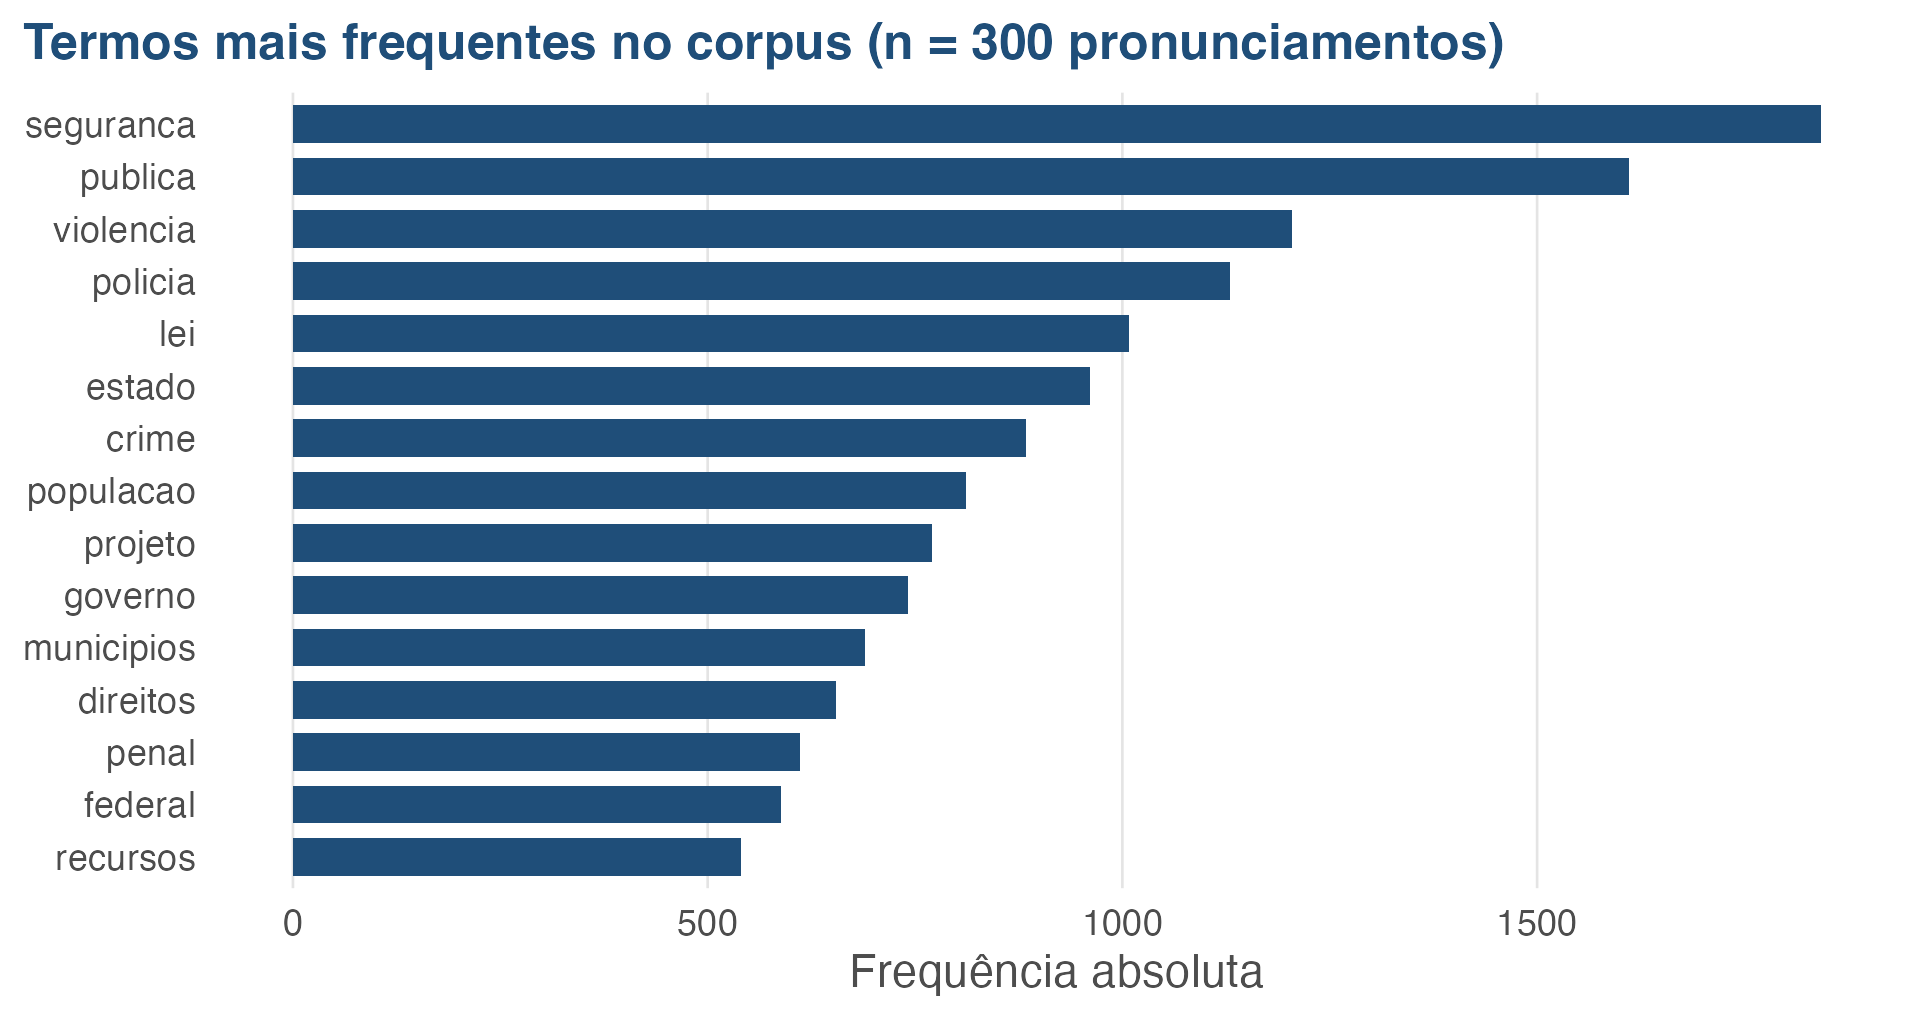
\includegraphics[width=\linewidth]{figuras/fig_top_terms.png}
\end{columns}
\end{frame}

\begin{frame}[fragile]{Demo 3. Descrever: distintividade entre grupos}
\begin{columns}[T]
\column{0.44\textwidth}
\begin{lstlisting}
# TF-IDF: o que e DISTINTIVO
freq_partido <- ac_count(corpus_limpo,
                         by = "partido")
tfidf <- ac_tf_idf(freq_partido,
                   by = "partido")

# Keyness: teste estatistico
kn <- ac_keyness(freq_partido,
                 group  = "partido",
                 target = "PT")
ac_plot_keyness(kn)
\end{lstlisting}
\vspace{0.1cm}
\footnotesize \textbf{Keyness} compara a frequência observada de cada termo no
grupo-alvo com a esperada sob o grupo de referência.
\column{0.55\textwidth}
\centering
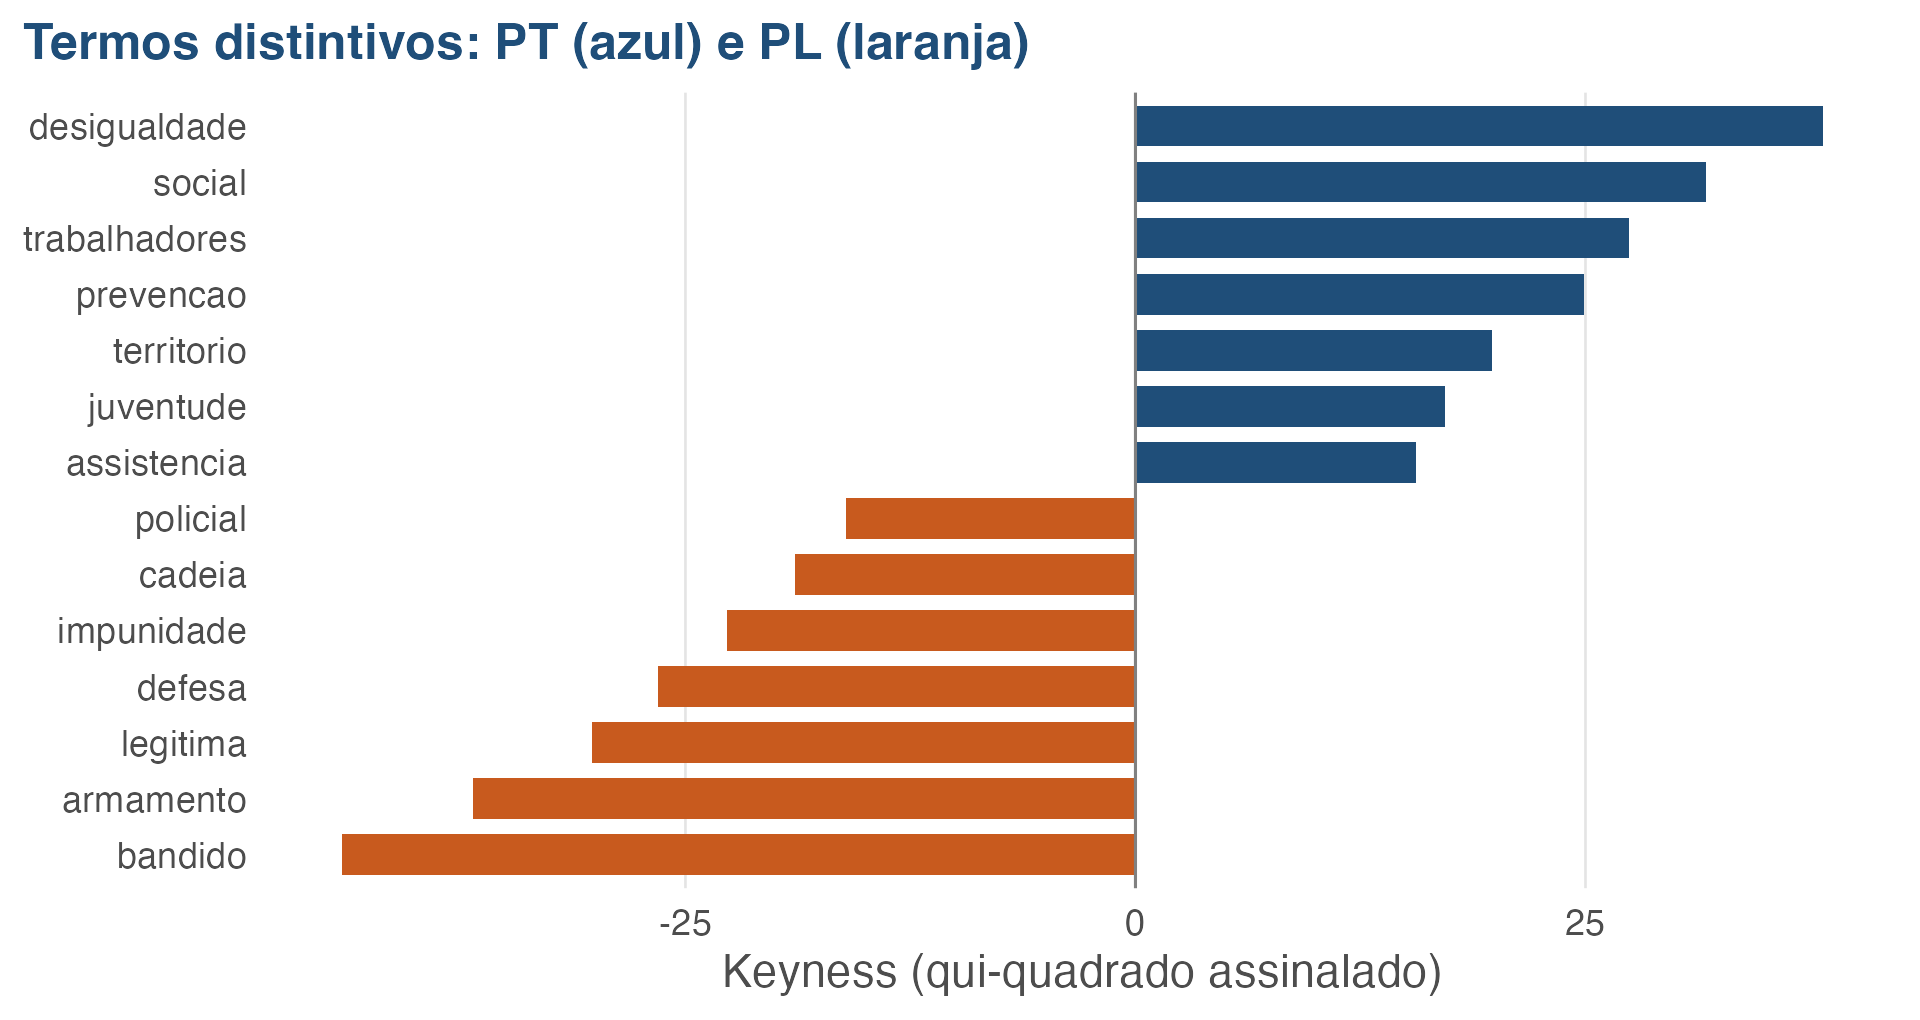
\includegraphics[width=\linewidth]{figuras/fig_keyness.png}\\
\scriptsize \textit{Saída ilustrativa, gerada para fins didáticos.}
\end{columns}
\end{frame}

\begin{frame}{Interpretando a saída: três perguntas obrigatórias}
Diante de qualquer tabela de frequência ou de \emph{keyness}:
\vspace{0.3cm}
\begin{enumerate}
  \item \textbf{Quem produziu esses termos?}\\
        \small Verifique concentração por autor. Um deputado com 400
        pronunciamentos domina qualquer contagem agregada.
  \vspace{0.15cm}
  \item \normalsize \textbf{O termo significa a mesma coisa nos dois grupos?}\\
        \small ``Reforma'' em 1995 e em 2019 não são o mesmo objeto. Comparar
        períodos exige atenção ao deslocamento semântico.
  \vspace{0.15cm}
  \item \normalsize \textbf{O que eu esperaria ver se minha hipótese fosse falsa?}\\
        \small Sem essa resposta, qualquer lista de palavras confirma qualquer
        narrativa.
\end{enumerate}
\end{frame}

\begin{frame}[fragile]{A ferramenta de disciplina: voltar ao texto}
\begin{lstlisting}
# KWIC: onde e como o termo aparece, no contexto original
library(quanteda)
tokens_qt <- quanteda::tokens(corpus_limpo$text)
kwic(tokens_qt, pattern = "impunidade", window = 6) |> head(4)
\end{lstlisting}
\begin{lstlisting}[style=Rsaida]
 docname       pre                        keyword       post
 disc-000912  "a sensacao de"             impunidade   "que toma conta do pais"
 disc-001044  "combater a"                impunidade   "significa investir em"
 disc-001156  "falar em"                  impunidade   "sem falar em desigualdade"
 disc-001203  "o discurso da"             impunidade   "serve para justificar"
\end{lstlisting}
\vspace{0.2cm}
\begin{alertblock}{Note o que aconteceu}
\small O mesmo termo aparece em posições argumentativas \textbf{opostas}. Uma
contagem agregada trataria os quatro casos como equivalentes. Custa dois minutos
verificar, e evita uma conclusão falsa.
\end{alertblock}
\end{frame}

\begin{frame}[fragile]{Demo 4. Descobrir: modelagem de tópicos}
\begin{columns}[T]
\column{0.40\textwidth}
\begin{lstlisting}
# SEMPRE fixe a seed
lda <- ac_lda(corpus_limpo,
              k = 4,
              seed = 1234)

ac_plot_lda_topics(lda)
\end{lstlisting}
\vspace{0.15cm}
\footnotesize O LDA trata cada documento como mistura de $k$ tópicos latentes, e
cada tópico como distribuição sobre palavras.
\vspace{0.1cm}

\scriptsize \textit{Saída ilustrativa, gerada para fins didáticos.}
\column{0.59\textwidth}
\centering
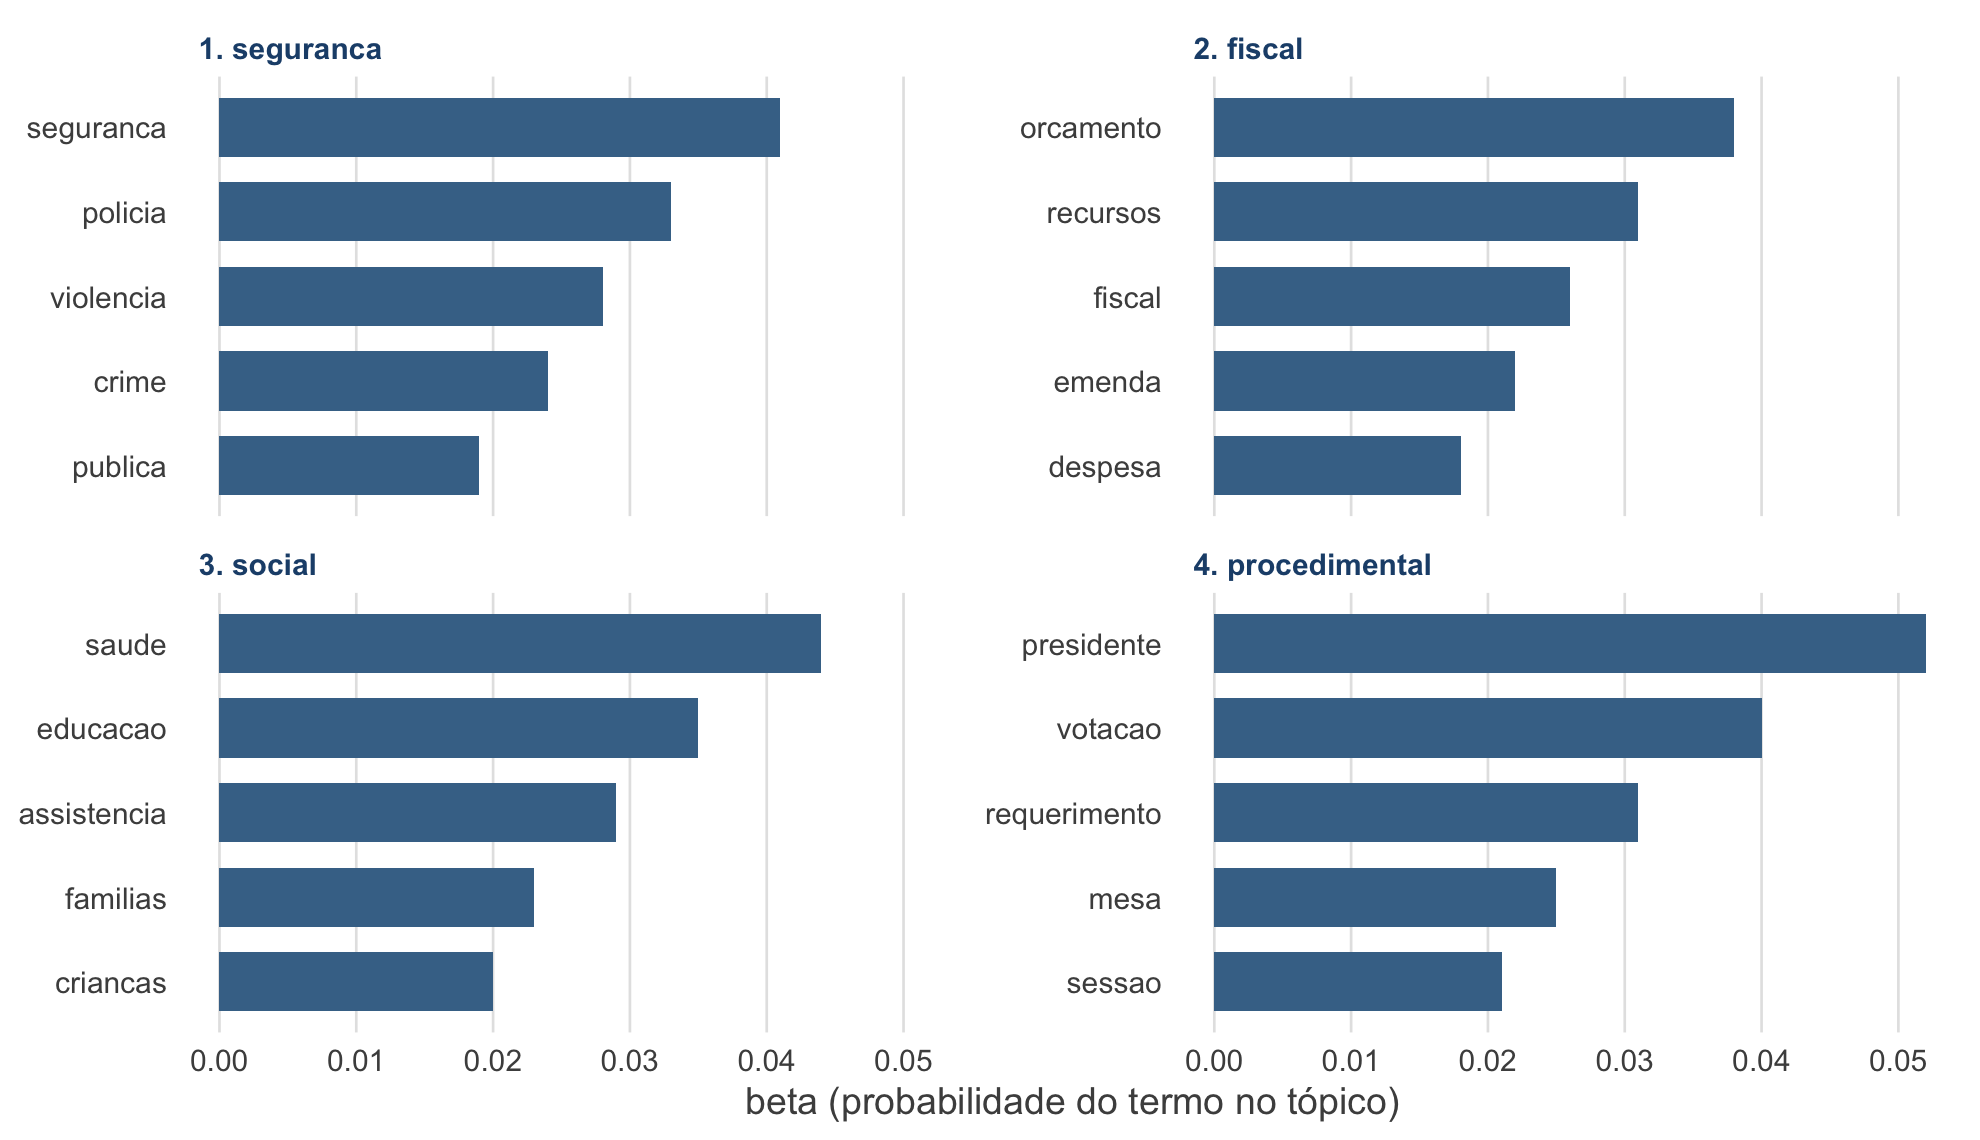
\includegraphics[width=\linewidth]{figuras/fig_lda.png}
\end{columns}
\vspace{0.1cm}
\footnotesize \textbf{Repare no Tópico 4:} ele capturou vocabulário
procedimental, não substantivo. Isso é comum e precisa ser reportado.
\end{frame}

\begin{frame}{A armadilha do $k$}
\begin{alertblock}{Não existe $k$ correto}
Métricas de coerência e exclusividade ajudam a delimitar uma faixa razoável, mas
a decisão final é interpretativa e é sua.
\end{alertblock}
\vspace{0.35cm}
\textbf{O passo mais frágil de toda a literatura aplicada:} nomear os tópicos
lendo as dez palavras mais prováveis.
\vspace{0.25cm}
\begin{itemize}
  \item Nomear não é validar.
  \item A leitura das palavras principais gera uma narrativa plausível para
        praticamente qualquer conjunto de termos.
  \item O nome do tópico entra no artigo como se fosse um achado, quando é uma
        interpretação não testada.
\end{itemize}
\end{frame}

\begin{frame}{Como validar um modelo de tópicos: o mínimo aceitável}
\begin{enumerate}
  \item \textbf{Validação semântica.} Leia uma amostra aleatória dos documentos
        com maior probabilidade em cada tópico. O rótulo sobrevive à leitura?
  \vspace{0.12cm}
  \item \textbf{Teste de intrusão.} Insira uma palavra estranha entre as
        principais do tópico. Codificadores humanos a identificam? Se não, o
        tópico não é coerente.
  \vspace{0.12cm}
  \item \textbf{Validação preditiva.} O tópico se comporta como esperado diante
        de choques externos conhecidos, como eleição ou crise?
  \vspace{0.12cm}
  \item \textbf{Estabilidade.} O tópico sobrevive a mudanças de $k$, de
        \emph{seed} e de pré-processamento?
\end{enumerate}
\pause
\vspace{0.25cm}
\begin{block}{Padrão de reporte honesto}
\small ``Dos 20 tópicos estimados, 12 foram interpretáveis e 8 descartados como
ruído de vocabulário procedimental.'' Isso é ciência. Apresentar os 20 como se
todos significassem algo, não é.
\end{block}
\end{frame}

% =============================================================================
\section{Validação}
% =============================================================================

\begin{frame}{Validação não é etapa: é critério de existência}
\begin{block}{O ponto epistemológico da manhã}
Uma categoria que dois codificadores treinados não conseguem aplicar de forma
convergente \textbf{não existe como objeto intersubjetivo}. É leitura
idiossincrática com aparência de método.
\end{block}
\vspace{0.3cm}
Isso vale igualmente quando um dos codificadores é um algoritmo.
\vspace{0.3cm}
\centering
\begin{tikzpicture}[node distance=0.5cm]
  \node[bloco, minimum width=4.6cm] (a) {Categoria rara: 95\% ``não''.\\
        Dois codificadores desatentos\\marcam tudo como ``não''};
  \node[alerta, minimum width=4.6cm, right=1.0cm of a] (b) {Concordância bruta: 95\%.\\
        Informação sobre a categoria: \textbf{zero}};
  \draw[seta] (a) -- (b);
\end{tikzpicture}
\end{frame}

\begin{frame}{Métricas de confiabilidade: quando usar cada uma}
\begin{table}
\scriptsize
\begin{tabular}{p{2.0cm}p{4.0cm}p{3.7cm}p{3.0cm}}
\toprule
\textbf{Métrica} & \textbf{Quando usar} & \textbf{Corte de referência} &
\textbf{Fonte} \\
\midrule
$\kappa$ de Cohen & 2 codificadores, dados nominais &
$\geq 0{,}70$ publicável; $\geq 0{,}80$ seguro &
Cohen (1960); Landis e Koch (1977) \\
\addlinespace
$\kappa$ de Fleiss & 3 ou mais codificadores, nominais & Mesmos cortes &
Fleiss (1971) \\
\addlinespace
$\alpha$ de Krippendorff & $N$ codificadores, escalas mistas, dados faltantes &
$\geq 0{,}667$ mínimo; $\geq 0{,}80$ confortável &
Krippendorff (2018) \\
\addlinespace
AC1 de Gwet & Categorias desbalanceadas & $\geq 0{,}70$ & Gwet (2008) \\
\addlinespace
$F_1$ macro & Avaliação contra \emph{gold standard} &
Depende da tarefa & Literatura de ML \\
\bottomrule
\end{tabular}
\end{table}
\vspace{0.1cm}
\footnotesize Toda essa família de métricas existe para descontar a concordância
esperada pelo acaso. Elas diferem apenas em como estimam esse acaso.
\end{frame}

\begin{frame}{O paradoxo que você precisa conhecer antes de reportar $\kappa$}
\begin{block}{Feinstein e Cicchetti (1990)}
Com prevalência muito desbalanceada, é possível ter concordância bruta altíssima
e $\kappa$ próximo de zero, ou até negativo. O problema não está na codificação,
e sim na distribuição marginal.
\end{block}
\vspace{0.35cm}
\textbf{O que fazer quando isso acontece:}
\begin{enumerate}\small
  \item Reporte concordância bruta, $\kappa$ e AC1 em conjunto.
  \item Apresente a matriz de confusão, que mostra onde está o desacordo.
  \item Considere amostragem estratificada para as categorias raras no teste de
        confiabilidade.
  \item Nunca reporte apenas o número que favorece seu argumento.
\end{enumerate}
\vspace{0.2cm}
\footnotesize \textit{Para a tarde:} o \texttt{acR} calcula todas essas métricas
simultaneamente, com intervalo de confiança por \emph{bootstrap}.
\end{frame}

% =============================================================================
\section{Fronteira}
% =============================================================================

\begin{frame}{LLMs entram no pipeline: o que mudou}
\begin{itemize}
  \item Classificação \emph{zero-shot} e \emph{few-shot} com desempenho
        competitivo em várias tarefas de anotação (Gilardi, Alizadeh e Kubli,
        2023).
  \vspace{0.1cm}
  \item Queda acentuada no custo de construir dados rotulados, o gargalo
        histórico da classificação supervisionada.
  \vspace{0.1cm}
  \item O modelo pode justificar a decisão, o que torna a codificação auditável
        em linguagem natural.
  \vspace{0.1cm}
  \item Categorias complexas, que exigem inferência contextual, passam a ser
        tratáveis em escala.
\end{itemize}
\pause
\vspace{0.35cm}
\centering
\small Nada disso é pouco. Mas repare que todos os ganhos são de
\textbf{custo e cobertura}, não de \textbf{validade}.
\end{frame}

\begin{frame}{LLMs entram no pipeline: o que não mudou}
\begin{itemize}
  \item Você continua precisando de um codebook explícito.
  \item Você continua precisando de um \emph{gold standard} humano.
  \item Você continua precisando reportar concordância por categoria.
\end{itemize}
\vspace{0.35cm}
\begin{alertblock}{O problema técnico central, que veremos à tarde}
Os erros do modelo são \textbf{sistemáticos}, e não aleatórios. Usar rótulos de
LLM como se fossem observados enviesa coeficientes de regressão, e esse viés não
desaparece com $N$ maior.
\end{alertblock}
\vspace{0.3cm}
\centering
\small A literatura recente propõe correções que combinam uma amostra pequena
rotulada por humanos com uma amostra grande rotulada pela máquina.
\end{frame}

\begin{frame}{Riscos que exigem tratamento explícito no artigo (1 de 2)}
\begin{enumerate}
  \item \textbf{Não determinismo.}\\
        \small O mesmo \emph{prompt}, no mesmo modelo, em datas diferentes, pode
        gerar rótulos diferentes. Fixe versão do modelo, temperatura e
        \emph{seed} quando disponível, e reporte a data de execução.
  \vspace{0.2cm}
  \item \normalsize \textbf{Opacidade e contaminação.}\\
        \small Você não sabe o que há no treino. Contaminação com o próprio
        corpus é possível e, na prática, indetectável.
  \vspace{0.2cm}
  \item \normalsize \textbf{Viés de posição e de rótulo.}\\
        \small Modelos tendem a favorecer categorias listadas primeiro e rótulos
        mais frequentes na língua. Teste embaralhando a ordem das categorias.
\end{enumerate}
\end{frame}

\begin{frame}{Riscos que exigem tratamento explícito no artigo (2 de 2)}
\begin{enumerate}\setcounter{enumi}{3}
  \item \textbf{Deriva de versão.}\\
        \small O provedor atualiza o modelo e seu resultado deixa de replicar.
        Salve os \emph{outputs} brutos, e não apenas o código.
  \vspace{0.2cm}
  \item \normalsize \textbf{Custo financeiro e energético.}\\
        \small Reporte o volume de chamadas e o modelo usado. É informação
        metodológica, não detalhe administrativo.
\end{enumerate}
\vspace{0.4cm}
\begin{block}{Regra que proponho}
\small O \emph{output} bruto do modelo é \textbf{dado primário} e deve ser
depositado junto com o corpus, em Zenodo, OSF ou Dataverse. Sem isso, o trabalho
é irreplicável por construção.
\end{block}
\end{frame}

\begin{frame}{Mapa conceitual do workshop}
\centering
\begin{tikzpicture}[node distance=0.65cm and 0.5cm]
  \node[destaque, minimum width=3.2cm] (t) {Texto político\\em larga escala};
  \node[bloco, minimum width=3.0cm, below left=0.8cm and 0.6cm of t] (a)
       {Análise de conteúdo\\categorias e codebook};
  \node[bloco, minimum width=3.0cm, below right=0.8cm and 0.6cm of t] (b)
       {Métodos\\computacionais};
  \node[destaque, minimum width=3.0cm, below=2.1cm of t] (c) {\textbf{Validação}};
  \node[bloco, minimum width=2.6cm, below left=0.8cm and 0.5cm of c] (s)
       {Supervisionado\\$F_1$, $\kappa$};
  \node[bloco, minimum width=2.6cm, below=0.8cm of c] (n) {Não supervisionado\\LDA, STM};
  \node[bloco, minimum width=2.6cm, below right=0.8cm and 0.5cm of c] (l)
       {LLMs\\zero e few-shot};
  \draw[seta] (t) -- (a); \draw[seta] (t) -- (b);
  \draw[seta] (a) -- (c); \draw[seta] (b) -- (c);
  \draw[seta] (c) -- (s); \draw[seta] (c) -- (n); \draw[seta] (c) -- (l);
\end{tikzpicture}
\vspace{0.15cm}

\small A validação é o nó que sustenta todas as arestas. É por ela que a tarde
começa.
\end{frame}

\begin{frame}{Síntese da manhã}
\begin{enumerate}
  \item A análise automatizada de texto herda integralmente as exigências da
        análise de conteúdo clássica e acrescenta outras.
  \item Identifique sua tarefa (descrever, classificar, medir ou descobrir)
        antes de escolher a ferramenta.
  \item Pré-processamento é decisão teórica. Justifique, reporte e teste
        robustez.
  \item Nenhum resultado não supervisionado é interpretável sem validação
        semântica, de intrusão ou preditiva.
  \item LLMs reduzem o custo de rotular, não o de validar. O erro deles é
        sistemático.
\end{enumerate}
\vspace{0.25cm}
\begin{block}{Tarefa de dez minutos para o almoço}
\small
Escreva uma frase: \emph{``Na minha pesquisa, a unidade de registro é \_\_\_\_,
a categoria que preciso medir é \_\_\_\_ e ela seria validada por \_\_\_\_.''}
Vamos usar essa frase na atividade da tarde.
\end{block}
\end{frame}

% =============================================================================
\section*{Referências}
% =============================================================================

\begin{frame}{Referências: o cânone \emph{text-as-data}}
\scriptsize
\begin{block}{Leitura obrigatória para quem vai fazer}
GRIMMER, Justin; STEWART, Brandon M. Text as data: the promise and pitfalls of
automatic content analysis methods for political texts. \textit{Political
Analysis}, v. 21, n. 3, p. 267--297, 2013.\\[2pt]
GRIMMER, Justin; ROBERTS, Margaret E.; STEWART, Brandon M. \textbf{Text as Data:
a new framework for machine learning and the social sciences}. Princeton:
Princeton University Press, 2022.\\[2pt]
DENNY, Matthew J.; SPIRLING, Arthur. Text preprocessing for unsupervised
learning: why it matters, when it misleads, and what to do about it.
\textit{Political Analysis}, v. 26, n. 2, p. 168--189, 2018.
\end{block}
\begin{block}{Panoramas}
WILKERSON, John; CASAS, Andreu. Large-scale computerized text analysis in
political science: opportunities and challenges. \textit{Annual Review of
Political Science}, v. 20, p. 529--544, 2017.\\[2pt]
GENTZKOW, Matthew; KELLY, Bryan; TADDY, Matt. Text as data. \textit{Journal of
Economic Literature}, v. 57, n. 3, p. 535--574, 2019.\\[2pt]
SALGANIK, Matthew J. \textbf{Bit by Bit: social research in the digital age}.
Princeton: Princeton University Press, 2018.
\end{block}
\end{frame}

\begin{frame}{Referências: métodos específicos}
\scriptsize
\begin{block}{Escalonamento e classificação}
LAVER, Michael; BENOIT, Kenneth; GARRY, John. Extracting policy positions from
political texts using words as data. \textit{American Political Science Review},
v. 97, n. 2, p. 311--331, 2003.\\[2pt]
SLAPIN, Jonathan B.; PROKSCH, Sven-Oliver. A scaling model for estimating
time-series party positions from texts. \textit{American Journal of Political
Science}, v. 52, n. 3, p. 705--722, 2008.\\[2pt]
HOPKINS, Daniel J.; KING, Gary. A method of automated nonparametric content
analysis for social science. \textit{American Journal of Political Science},
v. 54, n. 1, p. 229--247, 2010.\\[2pt]
BARBERÁ, Pablo et al. Automated text classification of news articles: a
practical guide. \textit{Political Analysis}, v. 29, n. 1, p. 19--42, 2021.
\end{block}
\begin{block}{Tópicos e \emph{embeddings}}
ROBERTS, Margaret E. et al. Structural topic models for open-ended survey
responses. \textit{American Journal of Political Science}, v. 58, n. 4,
p. 1064--1082, 2014.\\[2pt]
RODRIGUEZ, Pedro L.; SPIRLING, Arthur. Word embeddings: what works, what
doesn't, and how to tell the difference for applied research. \textit{Journal of
Politics}, v. 84, n. 1, p. 101--115, 2022.
\end{block}
\end{frame}

\begin{frame}{Referências: análise de conteúdo e confiabilidade}
\scriptsize
\begin{block}{Fundamentos e manuais aplicados}
KRIPPENDORFF, Klaus. \textbf{Content Analysis: an introduction to its
methodology}. 4. ed. Thousand Oaks: Sage, 2018.\\[2pt]
NEUENDORF, Kimberly A. \textbf{The Content Analysis Guidebook}. 2. ed. Thousand
Oaks: Sage, 2017.\\[2pt]
SAMPAIO, Rafael Cardoso; LYCARIÃO, Diógenes. \textbf{Análise de conteúdo
categorial: manual de aplicação}. Brasília: Enap, 2021.\\[2pt]
BARDIN, Laurence. \textbf{Análise de Conteúdo}. São Paulo: Edições 70, 2011.
\end{block}
\begin{block}{Métricas de concordância}
COHEN, Jacob. A coefficient of agreement for nominal scales. \textit{Educational
and Psychological Measurement}, v. 20, n. 1, p. 37--46, 1960.\\[2pt]
LANDIS, J. Richard; KOCH, Gary G. The measurement of observer agreement for
categorical data. \textit{Biometrics}, v. 33, n. 1, p. 159--174, 1977.\\[2pt]
GWET, Kilem L. Computing inter-rater reliability and its variance in the
presence of high agreement. \textit{British Journal of Mathematical and
Statistical Psychology}, v. 61, n. 1, p. 29--48, 2008.
\end{block}
\end{frame}

\begin{frame}{Referências: o paradoxo do kappa}
\scriptsize
\begin{block}{Leitura essencial antes de reportar concordância}
FEINSTEIN, Alvan R.; CICCHETTI, Domenic V. High agreement but low kappa: I. The
problems of two paradoxes. \textit{Journal of Clinical Epidemiology}, v. 43,
n. 6, p. 543--549, 1990.\\[3pt]
CICCHETTI, Domenic V.; FEINSTEIN, Alvan R. High agreement but low kappa: II.
Resolving the paradoxes. \textit{Journal of Clinical Epidemiology}, v. 43, n. 6,
p. 551--558, 1990.\\[3pt]
GWET, Kilem L. \textbf{Handbook of Inter-Rater Reliability}. 4. ed.
Gaithersburg: Advanced Analytics, 2014.
\end{block}
\vspace{0.2cm}
\normalsize
\begin{block}{Por que separei esta referência}
\small Este é o problema que mais aparece em corpora políticos brasileiros, em
que a categoria de interesse costuma ser rara. Se você for reportar $\kappa$ com
prevalência abaixo de 10\%, leia os dois artigos antes.
\end{block}
\end{frame}

\begin{frame}{Referências: debate brasileiro, LLMs e software}
\scriptsize
\begin{block}{Produção brasileira}
IZUMI, Mauricio; MOREIRA, Davi. O texto como dado: desafios e oportunidades para
as ciências sociais. \textit{BIB — Revista Brasileira de Informação
Bibliográfica em Ciências Sociais}, n. 86, p. 138--174, 2018.\\[2pt]
SAMPAIO, Rafael Cardoso et al. Muita Bardin, pouca qualidade: uma avaliação
sobre as análises de conteúdo qualitativas no Brasil. \textit{Revista Pesquisa
Qualitativa}, v. 10, n. 25, p. 464--494, 2022.\\[2pt]
LOVEJOY, Jennette et al. Assessing the reporting of reliability in published
content analyses: 1985--2010. \textit{Communication Methods and Measures}, v. 8,
n. 3, p. 207--221, 2014.
\end{block}
\begin{block}{LLMs em anotação e software}
GILARDI, Fabrizio; ALIZADEH, Meysam; KUBLI, Maël. ChatGPT outperforms crowd
workers for text-annotation tasks. \textit{PNAS}, v. 120, n. 30, 2023.\\[2pt]
BENOIT, Kenneth et al. quanteda: an R package for the quantitative analysis of
textual data. \textit{Journal of Open Source Software}, v. 3, n. 30, 2018.\\[2pt]
HENRIQUE, Anderson. \textbf{acR}: análise de conteúdo em R. Pacote R versão
0.3.2, 2026. Disponível em: \url{https://ahenriquecp.com/acR/}.
\end{block}
\end{frame}

% --- ENCERRAMENTO -------------------------------------------------------------
\begin{frame}[plain]
\centering
\vspace{0.9cm}
{\Large \textbf{Intervalo para o almoço}}\\[0.45cm]
{\large Voltamos às 13h30, para a parte prática}\\[0.7cm]

\small
\parbox{0.8\textwidth}{\centering
\textbf{Antes de voltar:}\\[0.18cm]
1. Confirme que \texttt{library(acR)} roda sem erro.\\
2. Baixe o repositório do workshop.\\
3. Traga sua frase: unidade de registro, categoria e validação.}
\vspace{0.7cm}

\footnotesize
\url{github.com/andersonheri/sicss-brazil-2026-text}\\[0.45cm]

\parbox{0.85\textwidth}{\scriptsize
\textbf{Como citar:} HENRIQUE, Anderson. \textit{Análise Automatizada de Texto:
estado da arte, desenho de pesquisa e primeiros códigos em R}. 2026.
Apresentação em slides: material didático não publicado, elaborado para o
Summer Institute in Computational Social Science, Brazil (SICSS-Brazil 2026),
Fundação Getulio Vargas, Rio de Janeiro. CEM-USP / INCT QualiGov.}

\end{frame}

\end{document}
